\documentclass[a4paper]{article}


\usepackage[T1]{fontenc}    
\usepackage[utf8]{inputenc} 
\usepackage{textcomp}      
\date{} 					
\author{}                   
\usepackage{geometry}		
\geometry{ left=2cm, right=2cm, top=2cm, bottom=4cm, bindingoffset=5mm}

\usepackage{graphicx}
\usepackage{xcolor}
\usepackage{hyperref} 
\usepackage{fancyhdr}												
\pagestyle{fancy}
\fancyhf{}
\fancyhead[R]{2973140 - Felix Bühler  \\ 2893121 - Jan Leusmann \\  3141241 - Jamie Ullerich}
\fancyhead[L]{Scientific Visualisation \\ Sommersemester 2019 }
\renewcommand{\headrulewidth}{0.5pt} 				

\title{Exercise 5}

\begin{document}

\maketitle 
\thispagestyle{fancy}



\section*{Exercise 5. 1 [3 Points] Delaunay Triangulation - Edge-Flip}

\begin{figure}[h!]
	\centering
	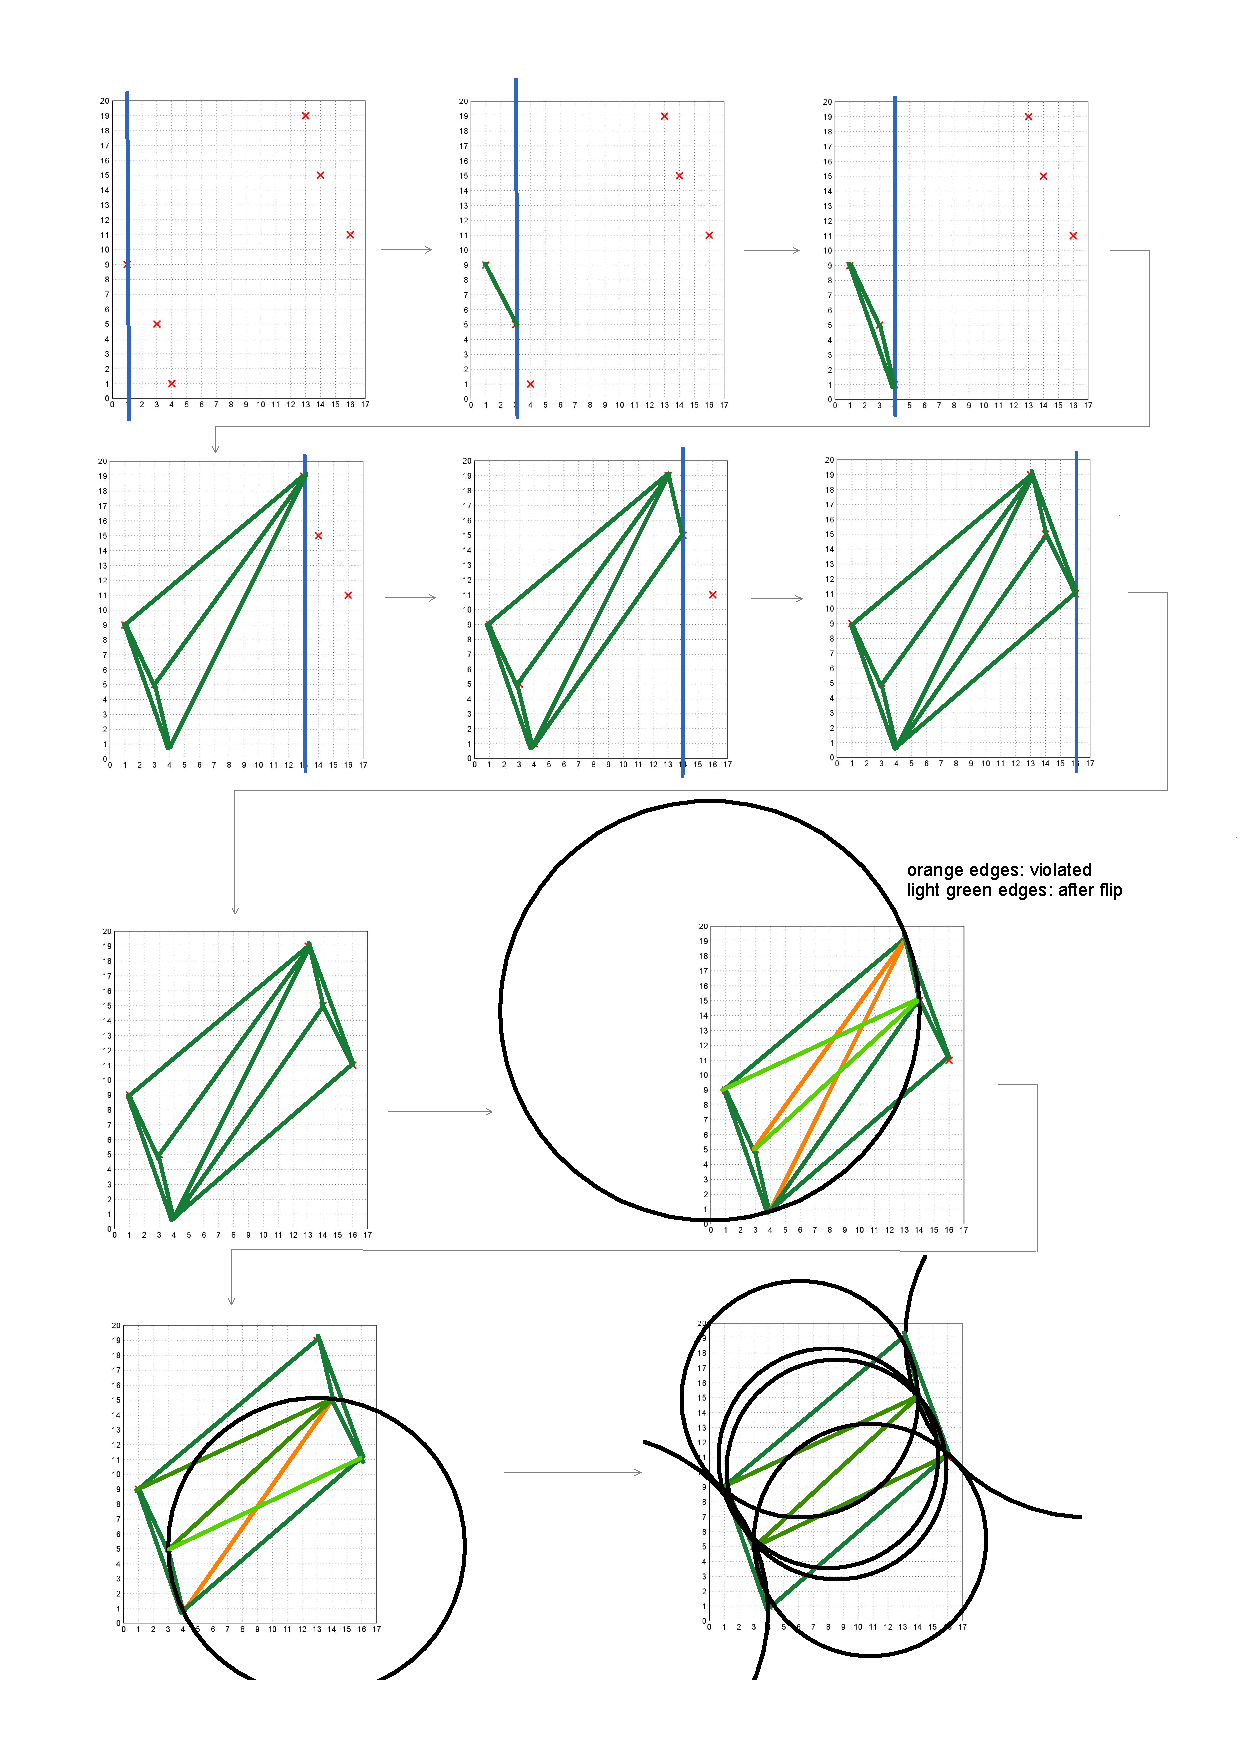
\includegraphics[width=0.79\linewidth]{delaunay.pdf}
	%\caption{}
	\label{fig:delaunay}
\end{figure}

\clearpage

\section*{Exercise 5. 2 [3 Points] Inverse Distance Weighting}
\begin{itemize}
	\item $ P_7 $:\\
	distances:
	\begin{itemize}
		\item $ P_1 $ = $ \sqrt{2} $
		\item $ P_2 $ = $ \sqrt{5} $
		\item $ P_3 $ = $ 1 $
		\item $ P_4 $ = $ \sqrt{8} $
	\end{itemize}
	\item $ P_8 $:\\
	distances:
	\begin{itemize}
		\item $ P_2 $ = $ 2.5 $
		\item $ P_3 $ = $ 1.5 $
		\item $ P_4 $ = $ \sqrt{4.25} $
		\item $ P_5 $ = $ 1.5 $
		\item $ P_6 $ = $ \sqrt{4.25} $
	\end{itemize}
\end{itemize}


\section*{Exercise 5. 3 [1 Points] Interpolation inside a prism}
	Get the inverse distance (eg. $ \frac{1}{distance} $) of point $ P $ and all corresponding. Then multiply the value of the point with the given result and sum all up.


\section*{Exercise 5. 4 [5 Points] Paraview: Simple Gradient Plugin}
--
	
\end{document}